\documentclass[12pt]{article}

\usepackage{amsmath}
\usepackage{titling}
\usepackage{lipsum}
\usepackage{graphicx}
\usepackage{tikz}

\graphicspath{ {img/} }

\title{A Proposed Model of the Short Run Returns of Studying}
\author{Bryan Bugyi}
\date{\today}

\pretitle{\begin{center}\Huge\bfseries}
\posttitle{\par\end{center}\vskip 0.5em}
\preauthor{\begin{center}\Large\ttfamily}
\postauthor{\end{center}}
\predate{\par\large\centering}
\postdate{\par}

\begin{document}
    \maketitle

    \begin{abstract}
        \lipsum[1]
    \end{abstract}

    \section{Introduction}
    As a student, it can be tempting to try to cram a week's worth of studies into a single day, or perhaps two. Any student who has tried this, however, is likely to have found that it is difficult to retain information this way. The first few hours of studying go as expected, but after that your ability to focus and actively engage with the material begins to wane. Subsequently, you don't remember as much of the material as you had hoped. In other words, you put in the hours, but it doesn't seem like they were used efficiently. This is not new information. The consequences of the law of diminishing returns are widely understood to reach far outside of their scope of modern economics; I would argue the principle has near universal relevance.
    
    While researching the subject, I came across several mathematical models that explain the phenomena of diminishing returns, most of which were exponential functions. For example, the function $f(x) = 3e^{\frac{-(x-15)}{20}}$, the graph of which is shown in Figure~\ref{Fig:Triv}, fits the bill quite nicely for a typical diminishing returns function. These relatively trivial exponential functions, however, do not in my opinion do a good job at modeling a human being's ability to focus.
    

    \begin{figure}[Htb]
        \begin{center}
            \caption{$f(x) = 3e^{\frac{-(x-15)}{20}}$} \label{Fig:Triv}
            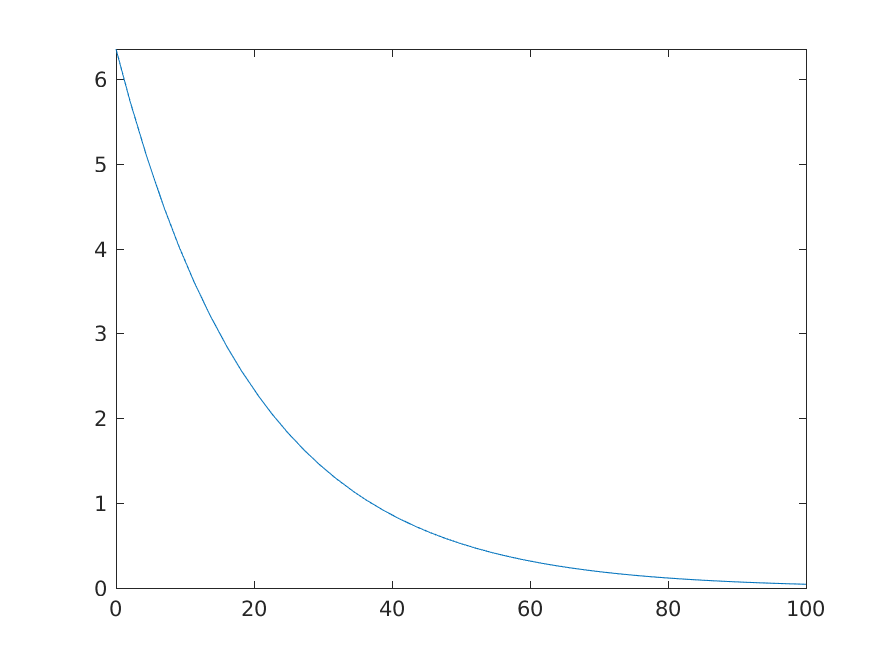
\includegraphics[scale=.5]{TrivialDimReturns.png}
        \end{center}
    \end{figure}

    This failure stems from the fact that the appropriate utility function would not be strictly decreasing. After all, when a study session first begins there is a great deal of inefficiency which results from our need to reorient ourselves to previous material. This is especially true when we begin reading a chapter that we have already partially read, start working on a problem set that we have already done work on previously, start working on project X where project X represents a partially complete project, etc.. 
    
    My intention in writing this paper (other than simply to organize my findings for later reference) is to demonstrate an example utility function that I believe provides a relatively accurate model of a human beings ability to study efficiently. After which, I will show how such a function could be used to maximize overall utility, which is, as I will go on to show, analogous to maximizing overall productivity.

    
    Such a model, if accurate, would not only provide an illustration of the phenomena of diminishing returns and its effects on our day-to-day lives but would also serve as a testament to the relevance of utility theory in cognitive research. This model could potentially even be applied to the effort of engineering a set of scheduling applications that work to effectively maximize total utility. Alternatively, through the use of this model, we may be able to better understand and potentially further validate focus and productivity software that is already in heavy use (e.g.\ the Pomodoro Method). 

    It should be noted that the model I am presenting is overly simplistic and is based only on my own personal introspection of my ability to focus on my studies for a given period of time. A successful, reliable model would be well tested and based on a sufficiently large, relevant dataset. Using this data and some form of nonlinear regression modeling, I have high hopes that an accurate model could be developed. This paper does not claim to have derived such a model, it only attempts to present what I believe to be the general form of such a model and also to demonstrate this model's potential utilization. To further reiterate this point, I believe it imperative that we clarify a few initial assumptions before moving forward. 

    \subsection*{Assumptions}

% \vspace{0.5cm}
\section*{Under Construction\ldots}
\begin{center}
    
\begin{tikzpicture}[limb/.style={line cap=round,line width=1.5mm,line join=bevel}]
        \draw[line width=2mm,rounded corners,fill=yellow] (-2,0) -- (0,-2) -- (2,0) -- (0,2) -- cycle;
        \fill (1.5mm,7mm) circle (1.5mm);
        \fill(0,-7.5mm) -- ++(10mm,0mm) -- ++(120:2mm)--++(100:1mm)--++(150:2mm) arc (70:170:2.5mm and 1mm);
        \draw[limb] (-7.5mm,-6.5mm)--++(70:4mm)--++(85:4mm) coordinate(a)--++(-45:5mm)--(-2.5mm,-6.5mm);
        \fill[rotate around={45:(a)}] ([shift={(-0.5mm,0.55mm)}]a) --++(0mm,-3mm)--++
            (7mm,-0.5mm)coordinate(b)--++(0mm,4mm)coordinate(c)--cycle;
        \draw[limb] ([shift={(-0.6mm,-0.4mm)}]b) --++(-120:5mm) ([shift={(-0.5mm,-0.5mm)}]c) --++
            (-3mm,0mm)--++(-100:3mm)coordinate (d);
        \draw[ultra thick] (d) -- ++(-45:1.25cm);
    \end{tikzpicture}
\end{center}

\end{document}
